\documentclass[10pt, twocolumn]{article}
%\pagestyle{plain}

\usepackage{amsfonts}
\usepackage{graphicx}


% This is how to make a comment

% These set the margins on your pages
%\hoffset=-1in
%\textwidth=6.5in
%\topmargin=0in
%\voffset=-0.75in
%\textheight=10in

\begin{document}



\title{SimHash: Hash-based Similarity Detection}

\author{Caitlin Sadowski\\
University of California, Santa Cruz\\
supertri@cs.ucsc.edu
\and
Greg Levin\\
University of California, Santa Cruz\\
glevin@cs.ucsc.edu}


%\date{}
\def\copyrightspace{}

\maketitle

\section{Abstract}


\section{Introduction}

As storage capacities become larger it is increasingly difficult to organize and manage growing file systems. Identical copies or older versions of files often become separated and scattered across a directory structure. Consolidating or removing multiple versions of a file becomes desirable. However, deduplication technologies do not extend well to the case where files are not identical. Techniques for identifying similar files could also be useful for classification purposes and as an aid to search.  A standard technique in similarity detection is to map features of a file into some high-dimensional space, and then use distance within this space as a measure of similarity.  Unfortunately, this typically involves computing the distance between all pairs of files, which leads to $O(n^2)$ similarity detection algorithms.  If these file-to-vector mappings could be reduced to a one-dimensional space, then the data points could be sorted in $O(n \log n)$ time, greatly increasing detection speed.

Our goal, then, would essentially be to create a `similarity hash function.''  Typically, hash functions are designed to minimize collisions (where two different inputs map to the same key value).  With cryptographic hash functions, collisions should be nearly impossible, and further, nearly identical data should hash to very different keys.  Our similarity hash function would have the opposite intent: very similar files should map to very similar, or even the same, hash key, and distance between keys should be some measure of the difference between files.  Of course, ``file size'' is a sort of hash function on files which satisfies these requirements.  However, while similar files are expected to have similar sizes, there is no expectation that just because two files have similar sizes that they should have similar content.  It is not at all clear how to condense information from a file into a more useful one-dimensional key.

While our project attempted this, we ended up relying on auxiliary data used in the eventual calculation of key values to refine our similarity tests.  Our key values are based on counting the occurrences of certain binary strings within a file, and combining these sums.  Unfortunately, the key values still end up being vaguely proportional to file size, and so many false positive matches are still generated.  However, our auxiliary data provides an easy and efficient means of refining our similarity detection.  A refined version of our keys based on file extension gives a much wider spread of key values, and alleviates some of the aforementioned problems.

\section{Semantics of Similarity}

"Similarity" is a vague word. We take the view that in order for two files to be similar they must share content. However, there are different ways to define that sharing. What about different encodings (ascii vs. unicode, WAV vs AIFF)? What if two files are different sizes, but one consists of, for example, repeated copies of the other one? 

Many previous attempts at file similarity detection have focused on detecting similarity on the \emph{text} \cite{hpDocRepositories, hoad} level. We decided to use \emph{binary} similarity as our metric. Two files are similar if only a small percentage of their raw bit patterns are different. We decided on binary similarity because we did not want to focus on one particular filetype (i.e. text documents) or structure. 

Another issue we do not explore is that of semantic similarity. For example, two text files may use different words but contain the same content in terms of meaning. We focus on syntactic, not semantic, similarity. In the words of Udi Manber, ``we make no effort to \emph{understand} the contents of the files.`` \cite{manber}

Broder \cite{broder} first made clear the distinction between \emph{resemblance} (when two files resemble each other) and \emph{containment} (when one file is contained inside of another). The focus of SimHash has been on resemblance detection. Two files with a size disparity (as in the example above) are implicitly different; Containment relationships between files do not necessarily make two files 'similar' under our metric.

In order for files to be similar under our type of metric, they must contain a large number of common pieces. Another dividing point is the granularity and coverage of these pieces. SimHash operates at a very fine granularity (byte or word level). We do not attempt complete coverage; we only care about the portions of the file which match our set of bit patterns.

Within some similarity metric, there needs to be a threshold to determine how close within the metric files need to be to count as similar. We are focused on files which have a strong degree of similarity, ideally within 1-2\% of each other.

Another issue is whether a form of similarity detection is meant to operate on a relative or absolute level. In other words, is the focus retrieving a set of files similar to a given file, or retrieving \emph{all} sets of similar files. SimHash does both.

% This is just an example of a figure......
 \begin{figure}[h] 
 \centering
%\includegraphics[height= 4.5in]{CritFig}
\caption{Sample Critical Path}
\label{CritDiag} 
\end{figure}    

\section{Implementation}

Our hash key is based on counting the occurrances of certain binary strings within a file.  The keys, along with certain intermediate data, are stored in a SQL database.  A separate program then queries the database for keys with similar values, and outputs the results.  The particulars of our method are described below.  Our code was written in C++, and developed simultaneously for Windows and Macintosh.  While the code runs equally well on both platforms, we used a Windows machine for primary development and a Mac for most data collection.

\subsection{Computing Hash Keys}

Since our notion of similarity is based on binary similarity, we start by counting the occurrances of various binary strings within the file.  We preselect a set of strings, called {\it Tags}, to search for.  We only use a subset of all possible strings of a given length, as summing matches over all strings would blur file differences.  String size was important, since shorter strings would not represent meaningful patterns, and longer strings would not be expected to occur with meaningful frequency in smaller files.  We chose to use 16 8-bit tags, although we experimented with several different sets of tags.

Our {\tt SimHash} program opens each file in a directory, scans through it, and looks for matches with each of our tags.  A count of matches, or {\it hits}, is kept for each tag, and these are stored in a {\it Sum Table}.  The hash key is then computed as a function of the sum table entries.  We restricted our attention to linear combinations of the sums, although we tried various weighting schemes.  Once this has all been computed, the file name, path, and size, along with its key and all entries in the sum table, are stored as a row in  a MySQL database.  Later on, we added the capacity to compute and store multiple keys per row, so that different sum table weightings could be compared side-by-side.

A variation of the key function was implemented to account for file extensions.  It is not unreasonable to claim that two files are inherently different if they contain different extensions.  Given this, it would be desirable for our hash function to assign very different values to any two files with different extensions.  To this end, we compute a simple hash of the (first three characters of) a file's extention, with a value between o and 1.  The distribution of these values should be fairly uniform across the space of possible extensions.  We then multiply this extension value by {\tt MAX\_INT}, and add that to our previous key value.  Since we only care about the {\it distance} between keys, and not their actual values, this will not affect the relation between files with the same extension, while it will tend to widely separate files of different extensions.  This has the effect of more evenly distributing our key values across the space of 32-bit integers, and making cross-extention key matches very unlikely.



\subsection{Finding Similarities}

Once the database has been populated with the data from a test directory, we use a second program called {\tt SimFind} to look for similar keys.  One file at a time, we perform a SQL query on its key to find all other key values within a certain tolerance range.  This is only the first level of our similarity filter.  For each file returned in this query, we then compute the distance between their sum tables, which is just the sum of the absolute values of the differences between their entries.  If this distance is within a certain tolerance, then we report the two files as similar.

Essentially, two files are deemed similar if they contain a very similar number of each of our selected tags in their bit patterns.  This method has several strengths and drawbacks.  Because the ordering of the tag matches within a file is not accounted for, rearranging the contents of a file will, up to a point, have little impact on key values and sum tables.  Similarly, adding or removing small pieces of a file will have only a small effect on these values.  Consequently, small changes to a file shouldn't throw off our similarity measure.  Further, the results of our calculations are relatively easy to understand and reason about.  Because ``similarity'' is based on the numerical distance between values, we can easily change the tolerance level for key and sum table distance matches.  Of course, increasing tolerance values both widens the range of similar files found and increases the number of false positives, so a good balance between these must be found.

On the downside, adding more than 1 or 2\% to a fil, will likely confound our notion of similarity, so new versions of files with significant additions will not be detected.  Also, as the order of strings within files is not measured, very different files can be detected as similar if they happen to share too many bit patterns.  In particular, the Law of Large Numbers makes false positives within our key space likely.  Since key similarity is the comparison that could be theoretically performed with an $O(\log n)$ search through a sorted list, an excess of false positives here means a larger number of pair-wise comparisons that must be performed on our sum table, even if those comparisons are computationally minimal.

\subsection{Resource Usage}

storage overhead

*offset so that we do not find the same string repeatedly (example of all 0's) 
*take filesize into account in our thresholds 
*cross platform compatibility
*identical files




\section{Results}

The first step of our analysis was to determine how different selections of tags and tag weights affected our results.  The second was to determine how well our scheme worked at detecting similar files and weeding out false positives.  For the first part, we found that an unbalanced scheme where only a few tags were used to compute a key worked best on a realistic file set, although different weighting schemes performed better on contrived data sets.  As for success, our scheme was successful at identifying files that fit our idea of similarity.  False positives were [...].

\subsection{Chosing Tags and Keys}

As mentioned above, we settled on 16 8-bit tags to apply our similarity measure.  In trying to select tags, we noticed that {\tt 0x00} was often the most significant single indicator of file structure.  This is not suprising, as some files are padded with large sections of zeros, while data rich files and text files contain few or no zero bytes.  Other than {\tt 0x00}, an essentially random selection of bytes values seem to perform generally better than contrived or structured tag sets.  We included the ASCII representations of 'e' and 't', as these appeared to be strong indicators of text-based data, and also non-ASCII range bytes which would not be less prevalent in text files.

We also investigated various relative weightings of tags in the calculation of the hash key.  We tried equal and unequal weightings of all tags, as well as giving zero weights to (i.e. ignoring) a large fraction of our tags.  On the whole, this last scheme performed best on real file sets. One measure of key performance was the ratio of key hits to sum table hits.  That is, what fraction of key hits are validated as as actually similar according to the sum table?  The lower this ratio, the lower the presumed false positive rate of the key.  [Figure 42 shows something like this]  Also in this graph, we can see the effects of the File Extention modification to our hash function.  This addition appears to weed out about [20\% of false positives].


[look at graphs, discuss in more detail]







 If the content of files were actually random, the Law of Large Numbers suggests the larger files would tend towards greater similarity, as the appearance of various tags would approach some mean.  

% This is just an example of a figure......
 \begin{figure}[h] 
 \centering
\includegraphics[width= 3in]{PairwiseElim.pdf}
\caption{Fractional reduction in the number of pairwise comparisions needed to establish similarity: Number of hits divided by n choose 2: }
\label{PairwiseSavings} 
\end{figure}    

 \begin{figure}[h] 
 \centering
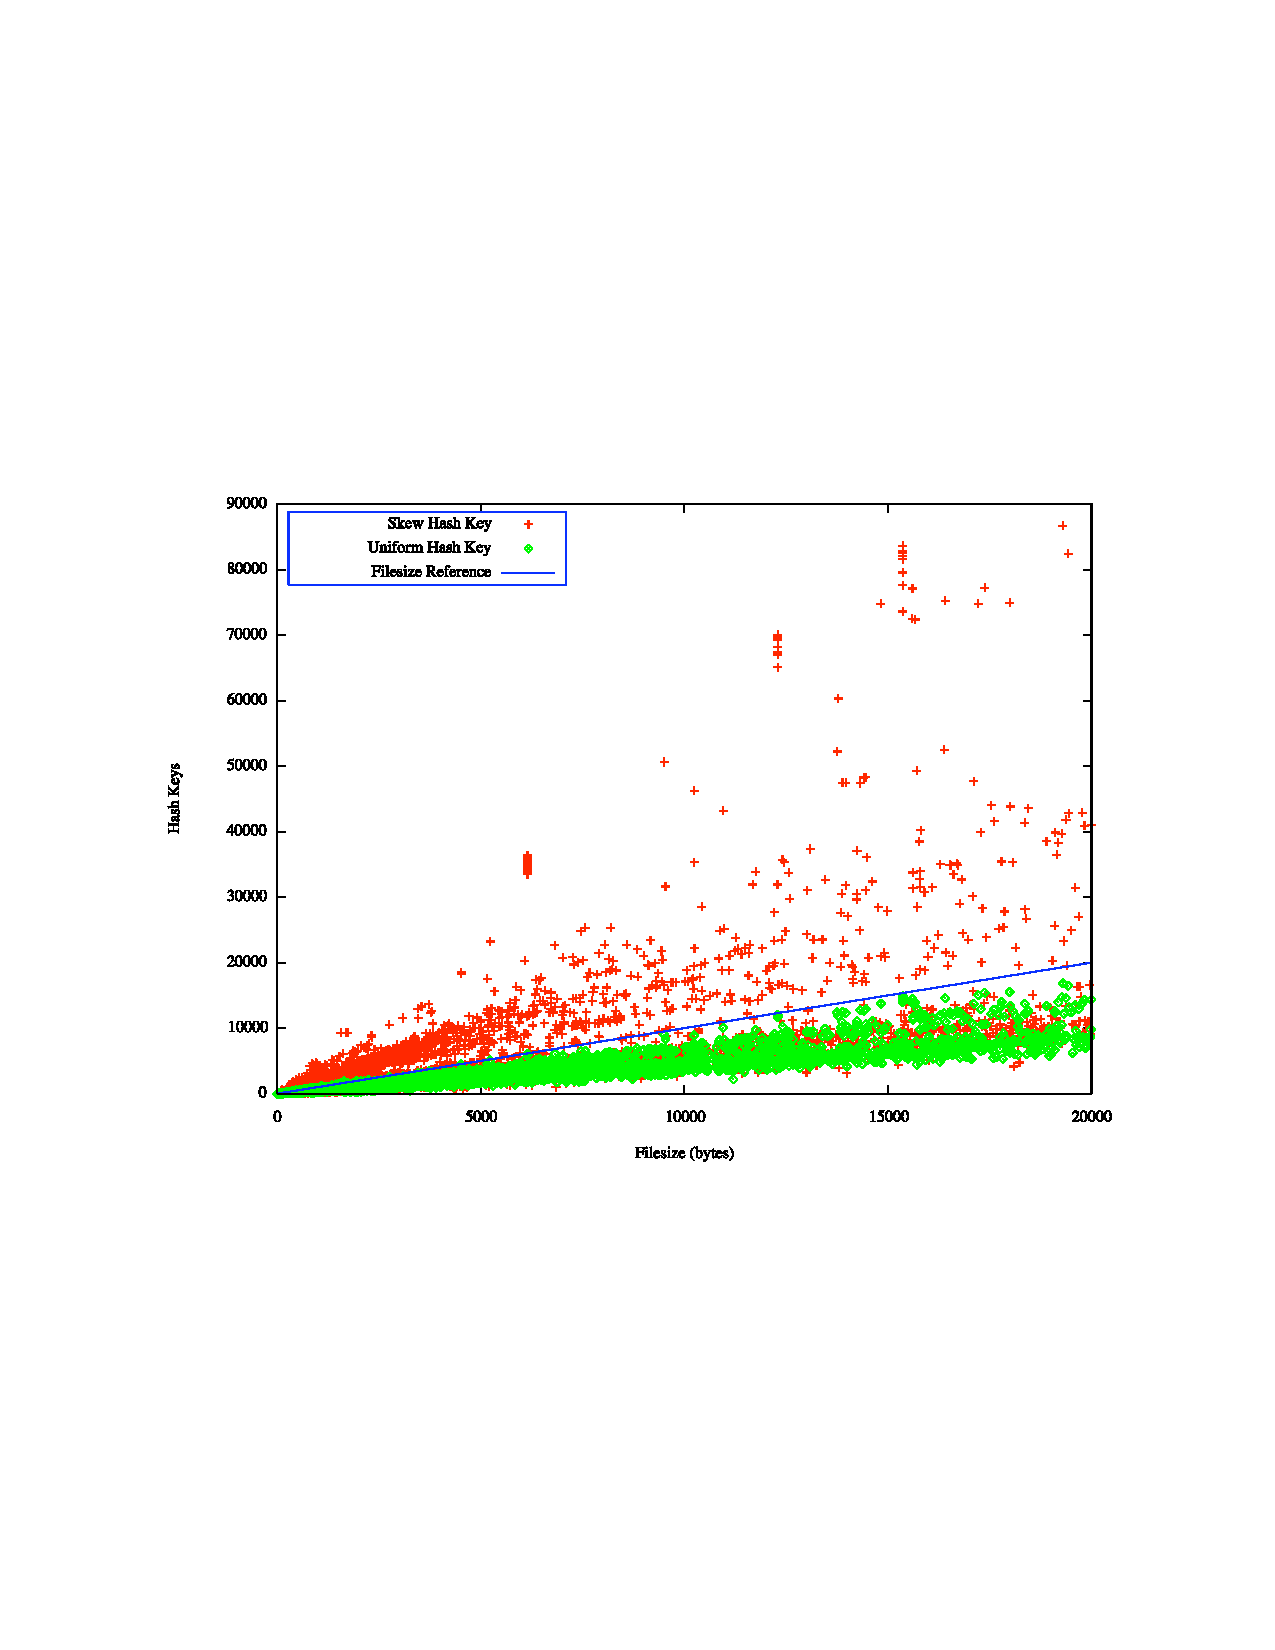
\includegraphics[width= 3in]{scatter_circles.pdf}
\caption{Visualization of Key Space with Uniform and Skewed weighting of sum table entries 
}
\label{scatterPoster} 
\end{figure}   

 \begin{figure}[h] 
 \centering
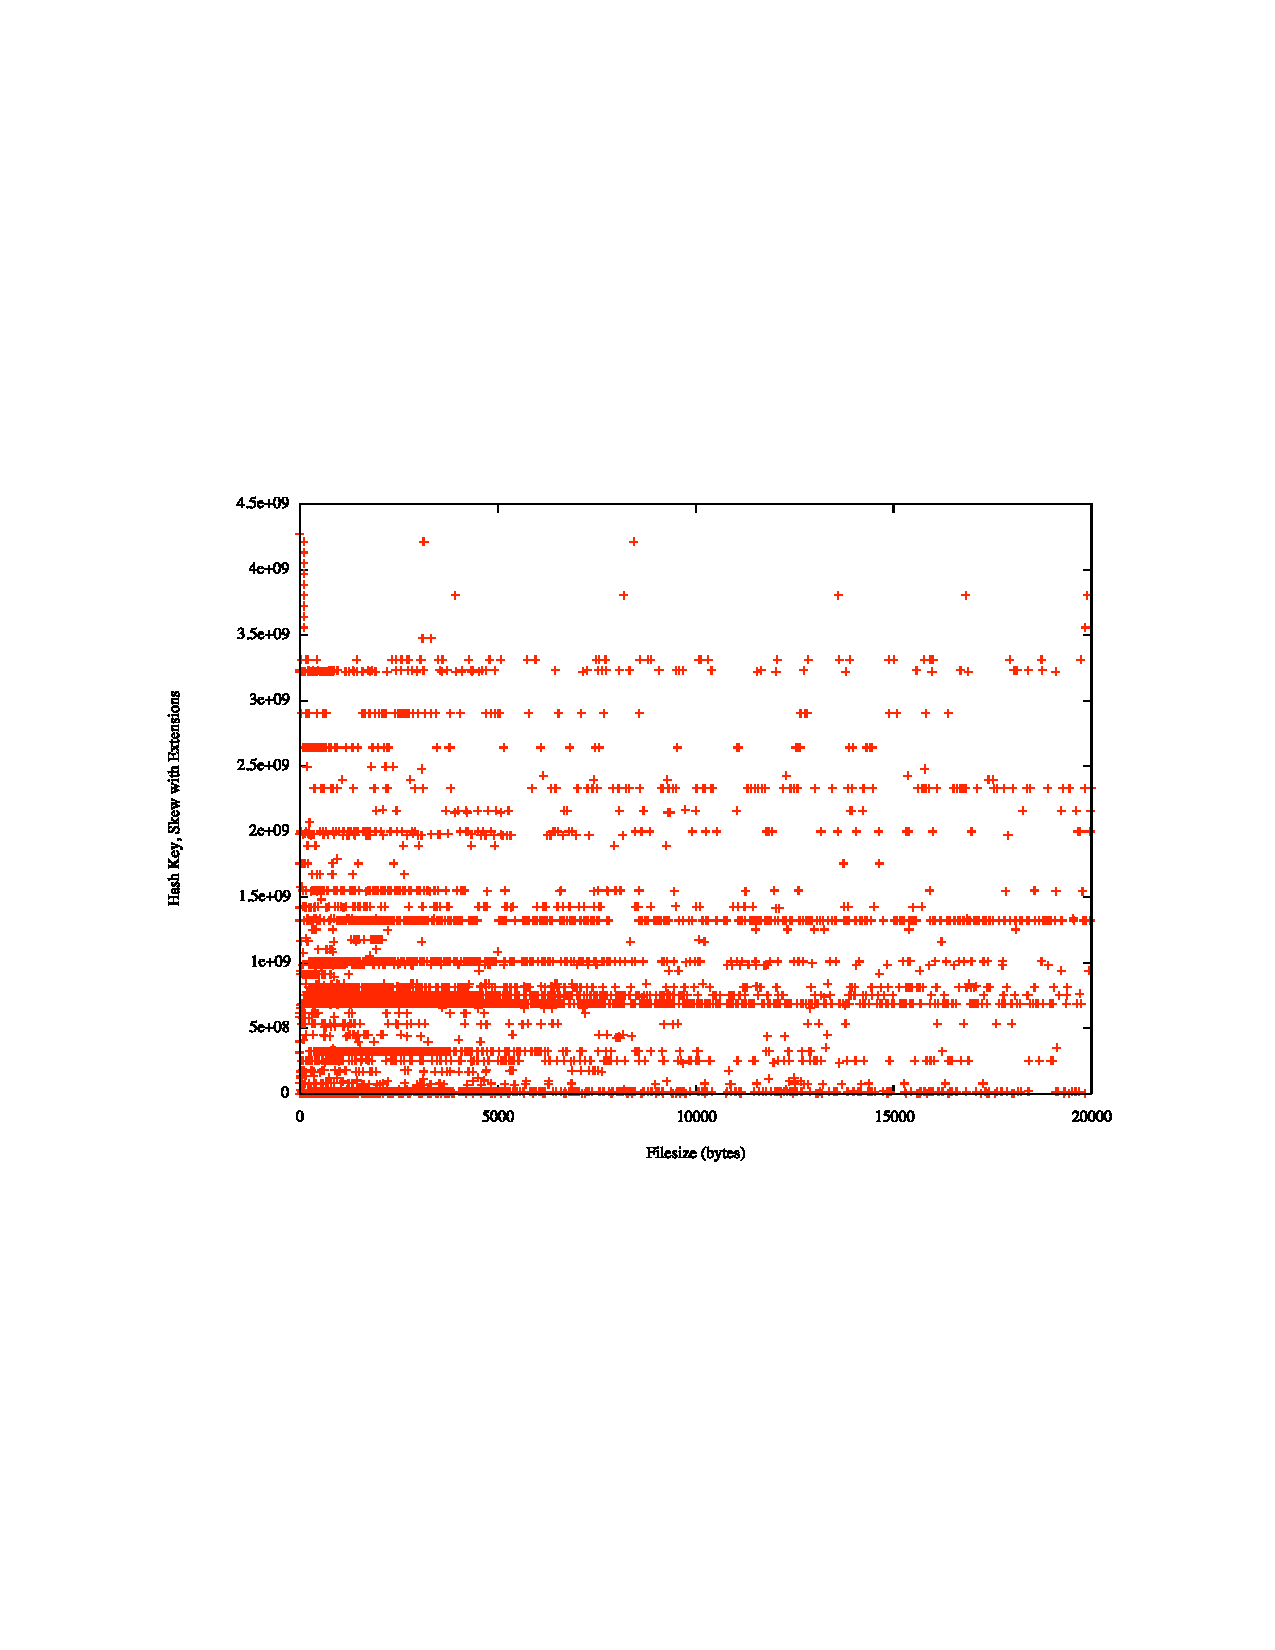
\includegraphics[width= 3in]{skewExtScatter.pdf}
\caption{Visualization of Key Space with Extensions factored into the Hash Key}
\label{scatterExtension} 
\end{figure}   

 \begin{figure}[h] 
 \centering
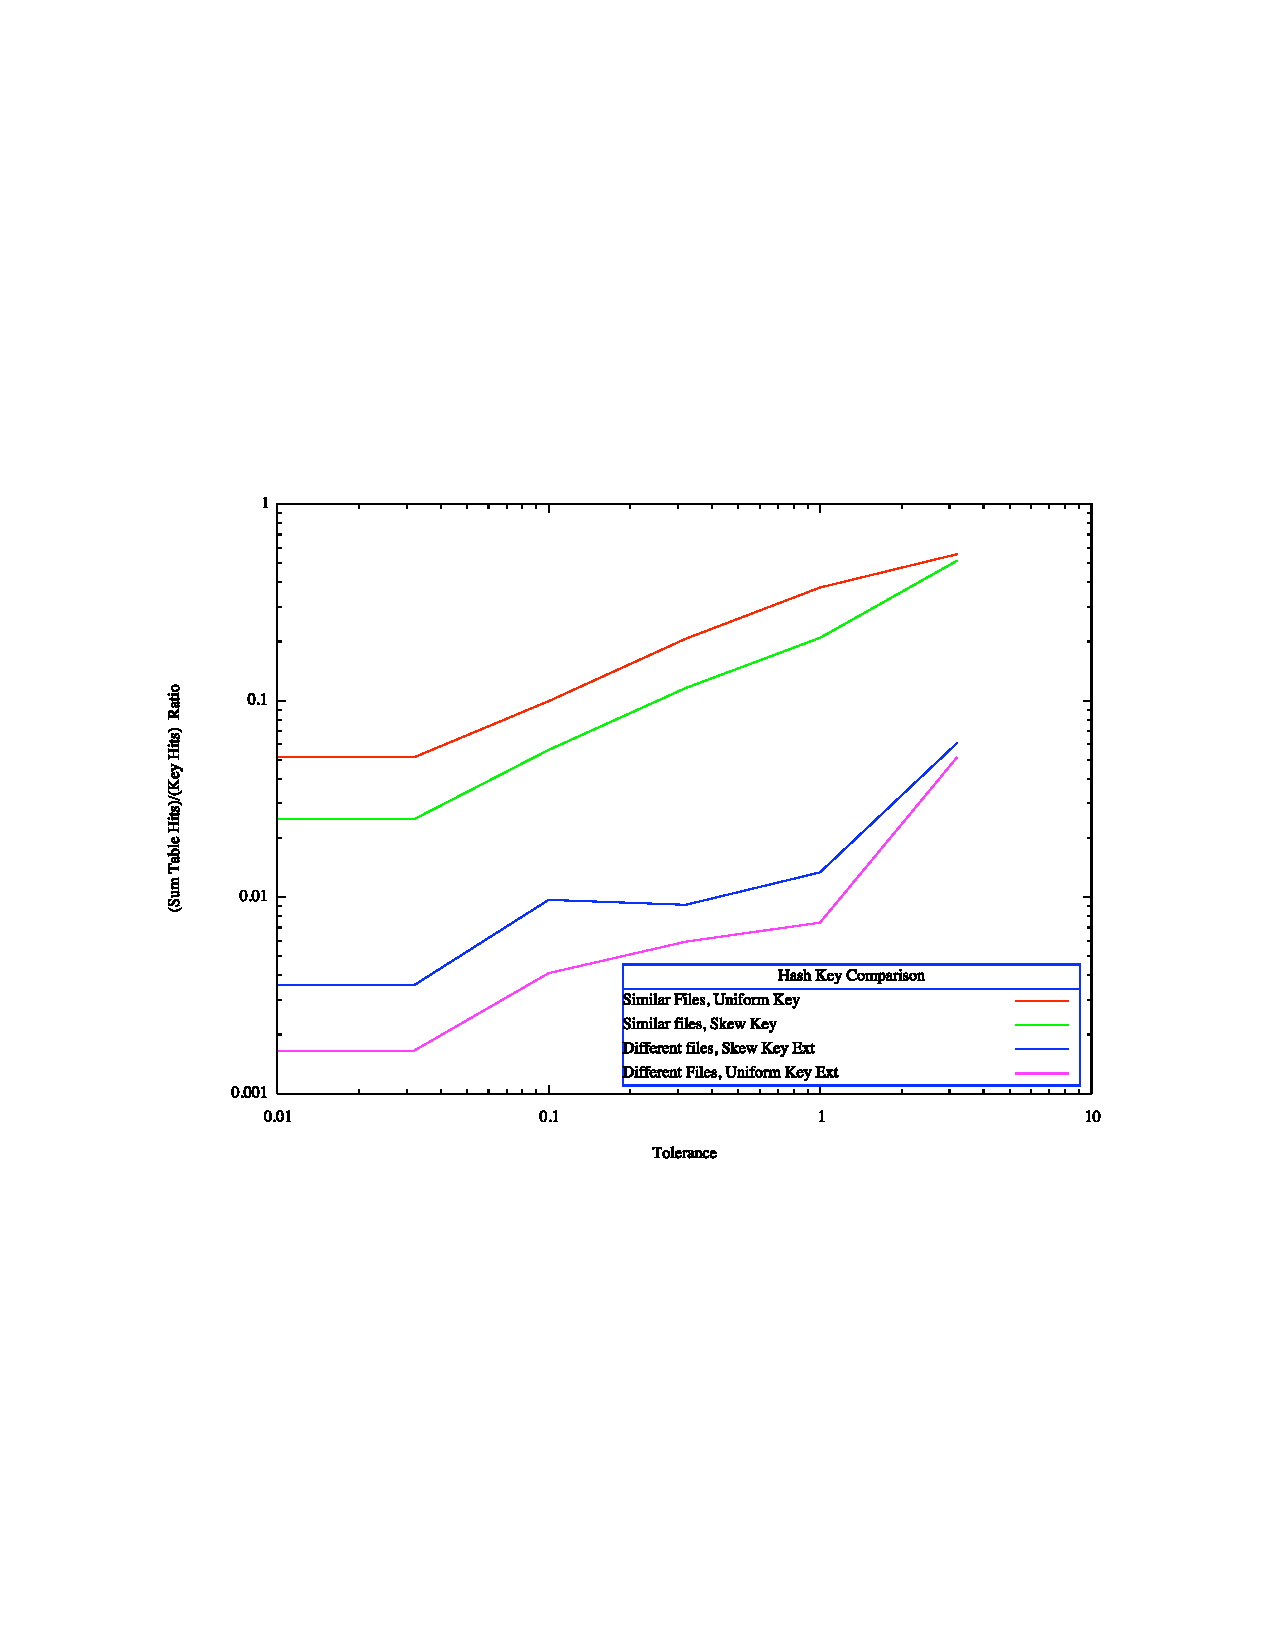
\includegraphics[width= 3in]{ratioSimDiff.pdf}
\caption{Comparing effectiveness of different key strategies on a predominantly similar or predominately different fileset.}
\label{simdiff} 
\end{figure}   

 \begin{figure}[h] 
 \centering
%\includegraphics[width= 3.5in]{PairwiseSavings_Cropped.pdf}
\caption{}
\label{performanceTest}
\end{figure}   

 \begin{figure}[h] 
 \centering
%\includegraphics[width= 3.5in]{PairwiseSavings_Cropped.pdf}
\caption{get together pdf/ps version!}
\label{headerFiles}
\end{figure}  

 \begin{figure}[h] 
 \centering
%\includegraphics[width= 3.5in]{PairwiseSavings_Cropped.pdf}
\caption{do the experiment}
\label{appendData}
\end{figure}  

%This is an example of a table...... 
% \begin{table}
 %\centering
  %\label{table1}
%\caption{New-Philo} 
%\medskip
 %\begin{tabular} {|c|c|} 
%\hline
%granularity & parallelism \\ \hline
%g = 1 & 1.367\\
%g = 10 & 3.226\\
%g = 100 & 3.186\\ \hline
%\end{tabular}
%\end{table}

\section{Related Work}

The problem of identifying file similarity is not a new one, although no one seems to have discovered a consistently good general solution. The most relevant paper to SimHash is over ten years old \cite{manber}. There has also been a body of research focusing on redundancy elimination, Much of the research on similarity detection since then has focused on very specific applications and filetypes. This includes:
\begin{itemize}
\item technical documentation \cite{hpDocRepositories} 
\item software systems \cite{sourcecode} 
\item plagiarism detection \cite{hoad} \cite{bernstein}
\item music \cite{music}
\item web pages \cite{buttler}
\end{itemize}

In most cases, the main goal of redundancy elimination is a reduction in either bandwidth or storage. Redundancy elimination (also "deduplication") can focus on eliminating multiple copies of the same file, or else preventing repeats of specific blocks shared between files. The standard way to identify duplicate blocks is by hashing each block. Venti \cite{venti} is an archival storage system which only stores only one copy of every block. As files are modified, new copies of modified blocks are written to disk, while unmodified blocks are still referenced. Shared or unmodified blocks are identified by comparing hashes of the blocks before writing to disk. LBFS \cite{lbfs} exemplifies a similar idea but focused on bandwidth reduction; when a file is changed, only modified blocks are sent over the network. If redundancy elimination is done at the block (or chunk) level, that provides a coarse-grained method of file similarity; files which share enough identical blocks are similar. Forman et al\cite{hpDocRepositories} took this approach when identifying similar documents in a repository. A natural question when classifying blocks is how to identify block boundaries. The options for this include fixed size chunking (for example, filesystem blocks), fixed size chunking over a sliding window (rsync \cite{rsync}), or some form of dynamic content-based chunking \cite{lbfs}. Content-defined chunking consistently outperforms fixed sized chunking at identifying redundancies, but involves larger time and space overheads  \cite{policroniades2004adr}.

Instead of looking for repeated blocks, delta-encoding works at a finer granularity. Essentially, it uses the difference (or delta) between two files to represent the second one. This is only effective when the two files resemble each other closely (for example, different versions in a version control system. DERD \cite{derd} investigates dynamically identifying similar files (or web pages) and then using delta-encoding to shrink the total footprint of similar pairs. The goal of REBL \cite{rebl} is heavy redundancy elimination with a combination of previous techniques. Identical and similar (content-based) chunks are identified. Identical chunks are removed, and similar chunks are delta-encoded. The remaining chunks are compressed, which essentially is redundancy elimination within one file.

Udi Manber \cite{manber} developed a technique for finding what he calls \emph{approximate fingerprints} of a file. His approach involves the concept of a set of \emph{anchors}, or small patterns of characters. In each file, a checksum of the characters around occurances of each anchor is computed. This set of checksums forms the fingerprints for the file, and is compared against fingerprints for other files when searching for similar files. Our sum table counts are in a similar vein. An important distinction between the two ideas is that we also form one hash key for each file to serve as an initial identification of similar files. 

\section{Future Work}

There are many ways to extend and build on the ideas presented here. We have experienced significant performance gains without losing possible matches when combining different hashkeys. We could be using a broader range of hashkeys.

Multiple similarity metrics for different filetypes could be combined to have a cohesive file similarity measure for the entire system.

There are few other metrics aside from binary similarity which would extend to the diversity of filetypes available in a system. One other example is metadata about files. We did not use file metadata for file similarity detection because we wanted our code to be cross-platform compatible. We also did not want to get caught up with issues of metadata reliability, and so limited our focus to the actual contents of the file. However, one could imagine adding heuristics for metadata similarity to the mix. 

bloom filters

\section{Conclusions}

\section{Acknowledgements}


% This MUST go at the end!
\end{document}